\FloatBarrier
\begin{figure}[!htb]
    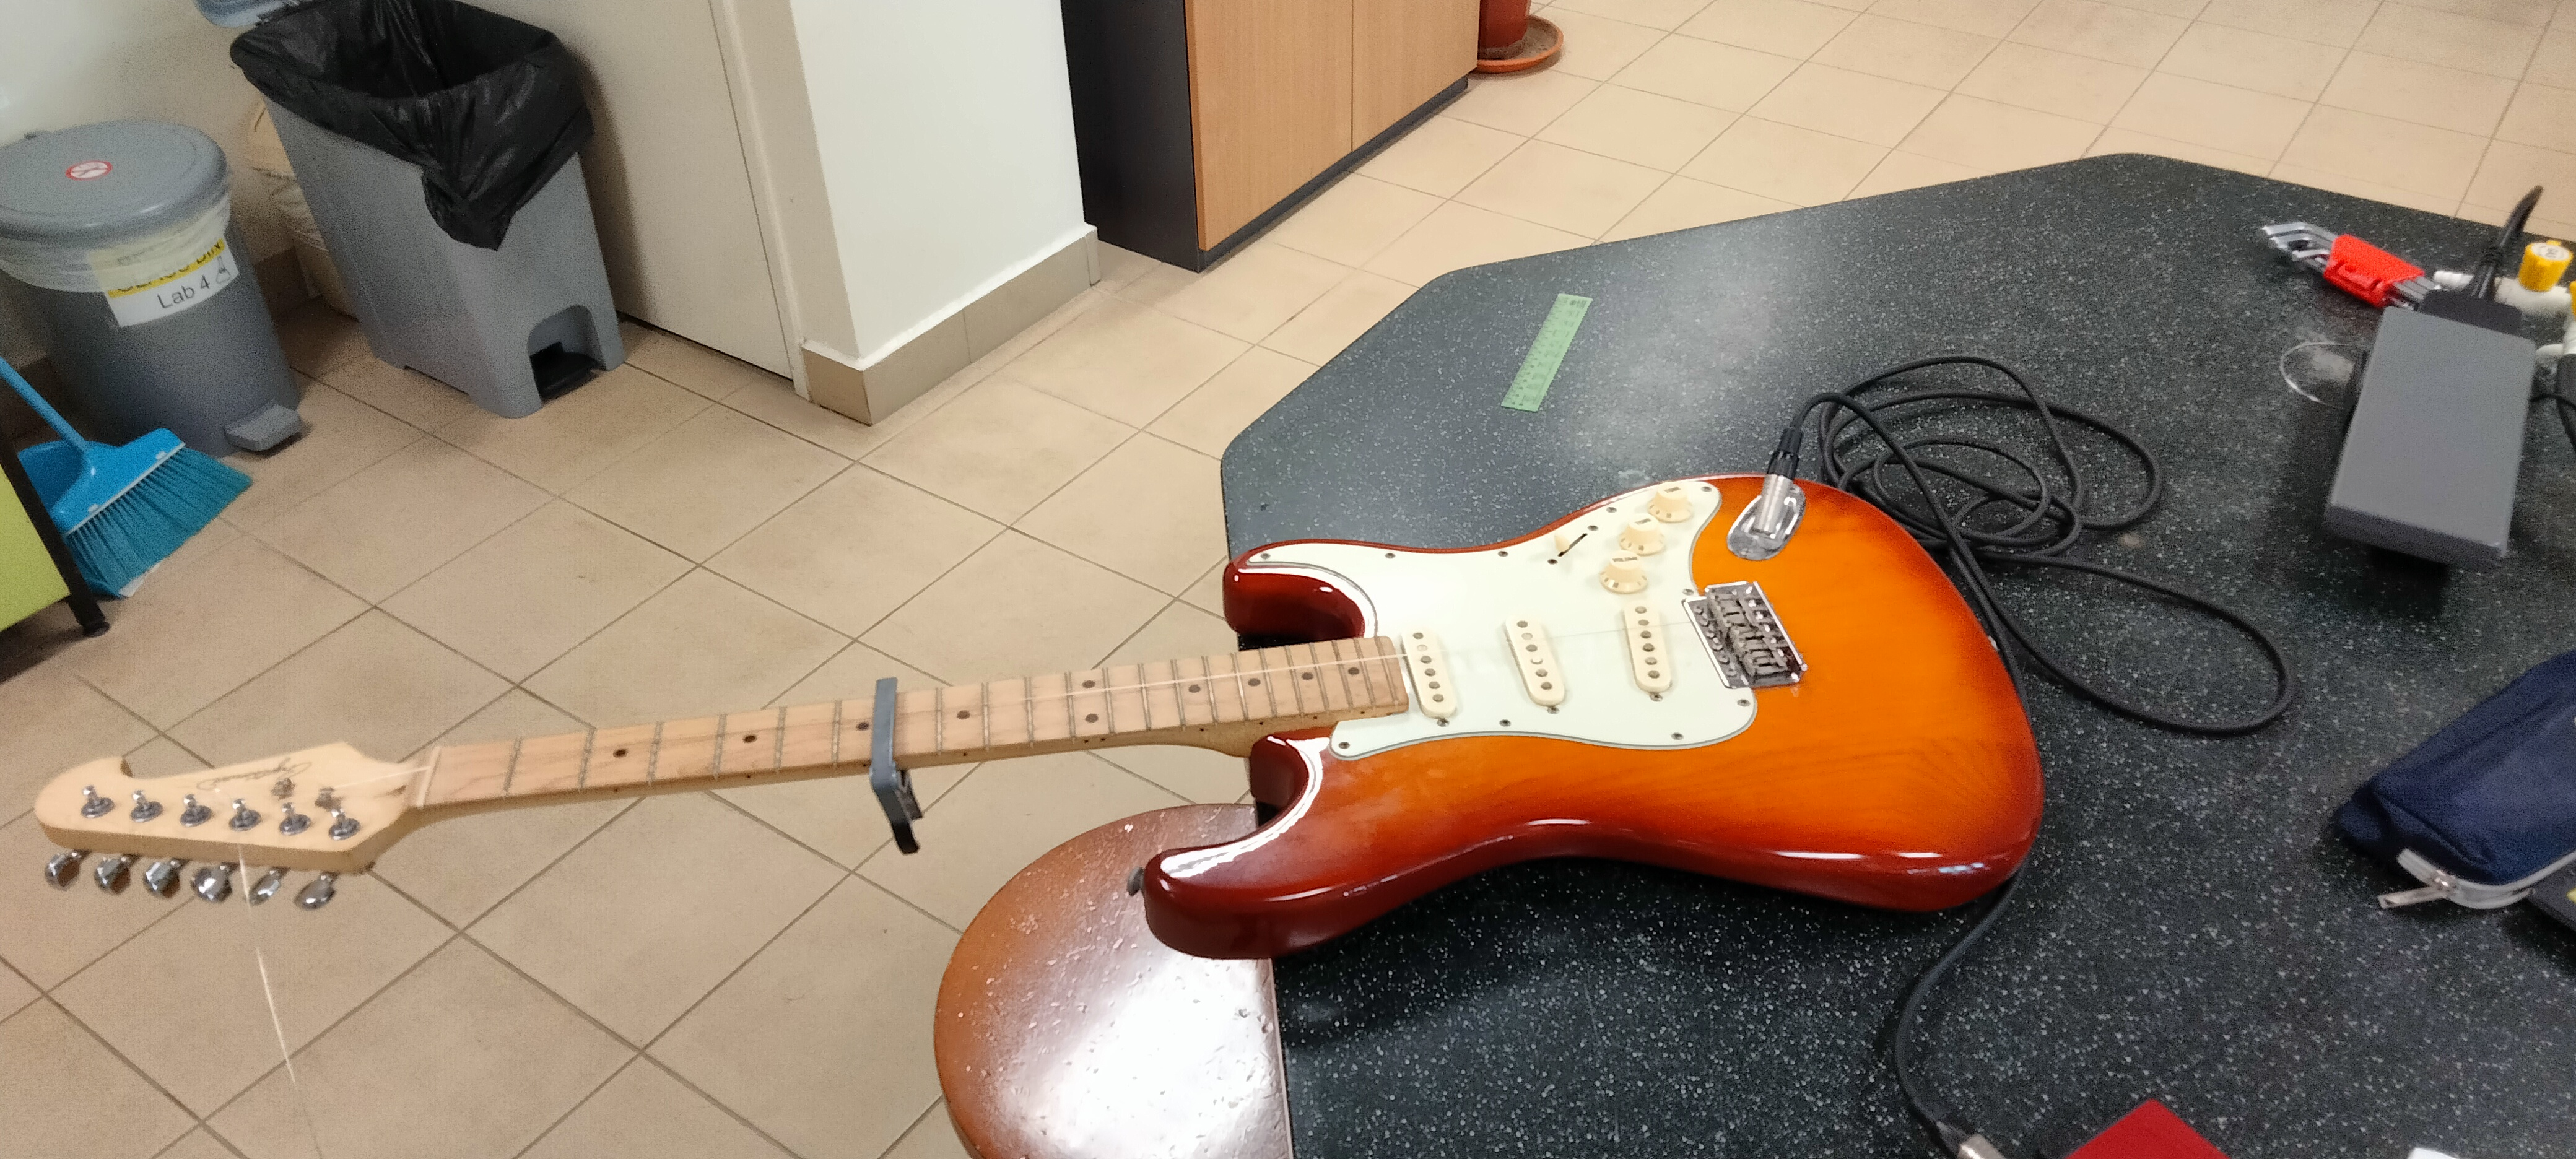
\includegraphics[width = \textwidth]{ee/experiment_setup.jpg}
    \caption{My experimental setup. I position the guitar neck outside the table for ease of access to the capo} \label{fig5}
\end{figure}
\begin{figure}[!htb]
    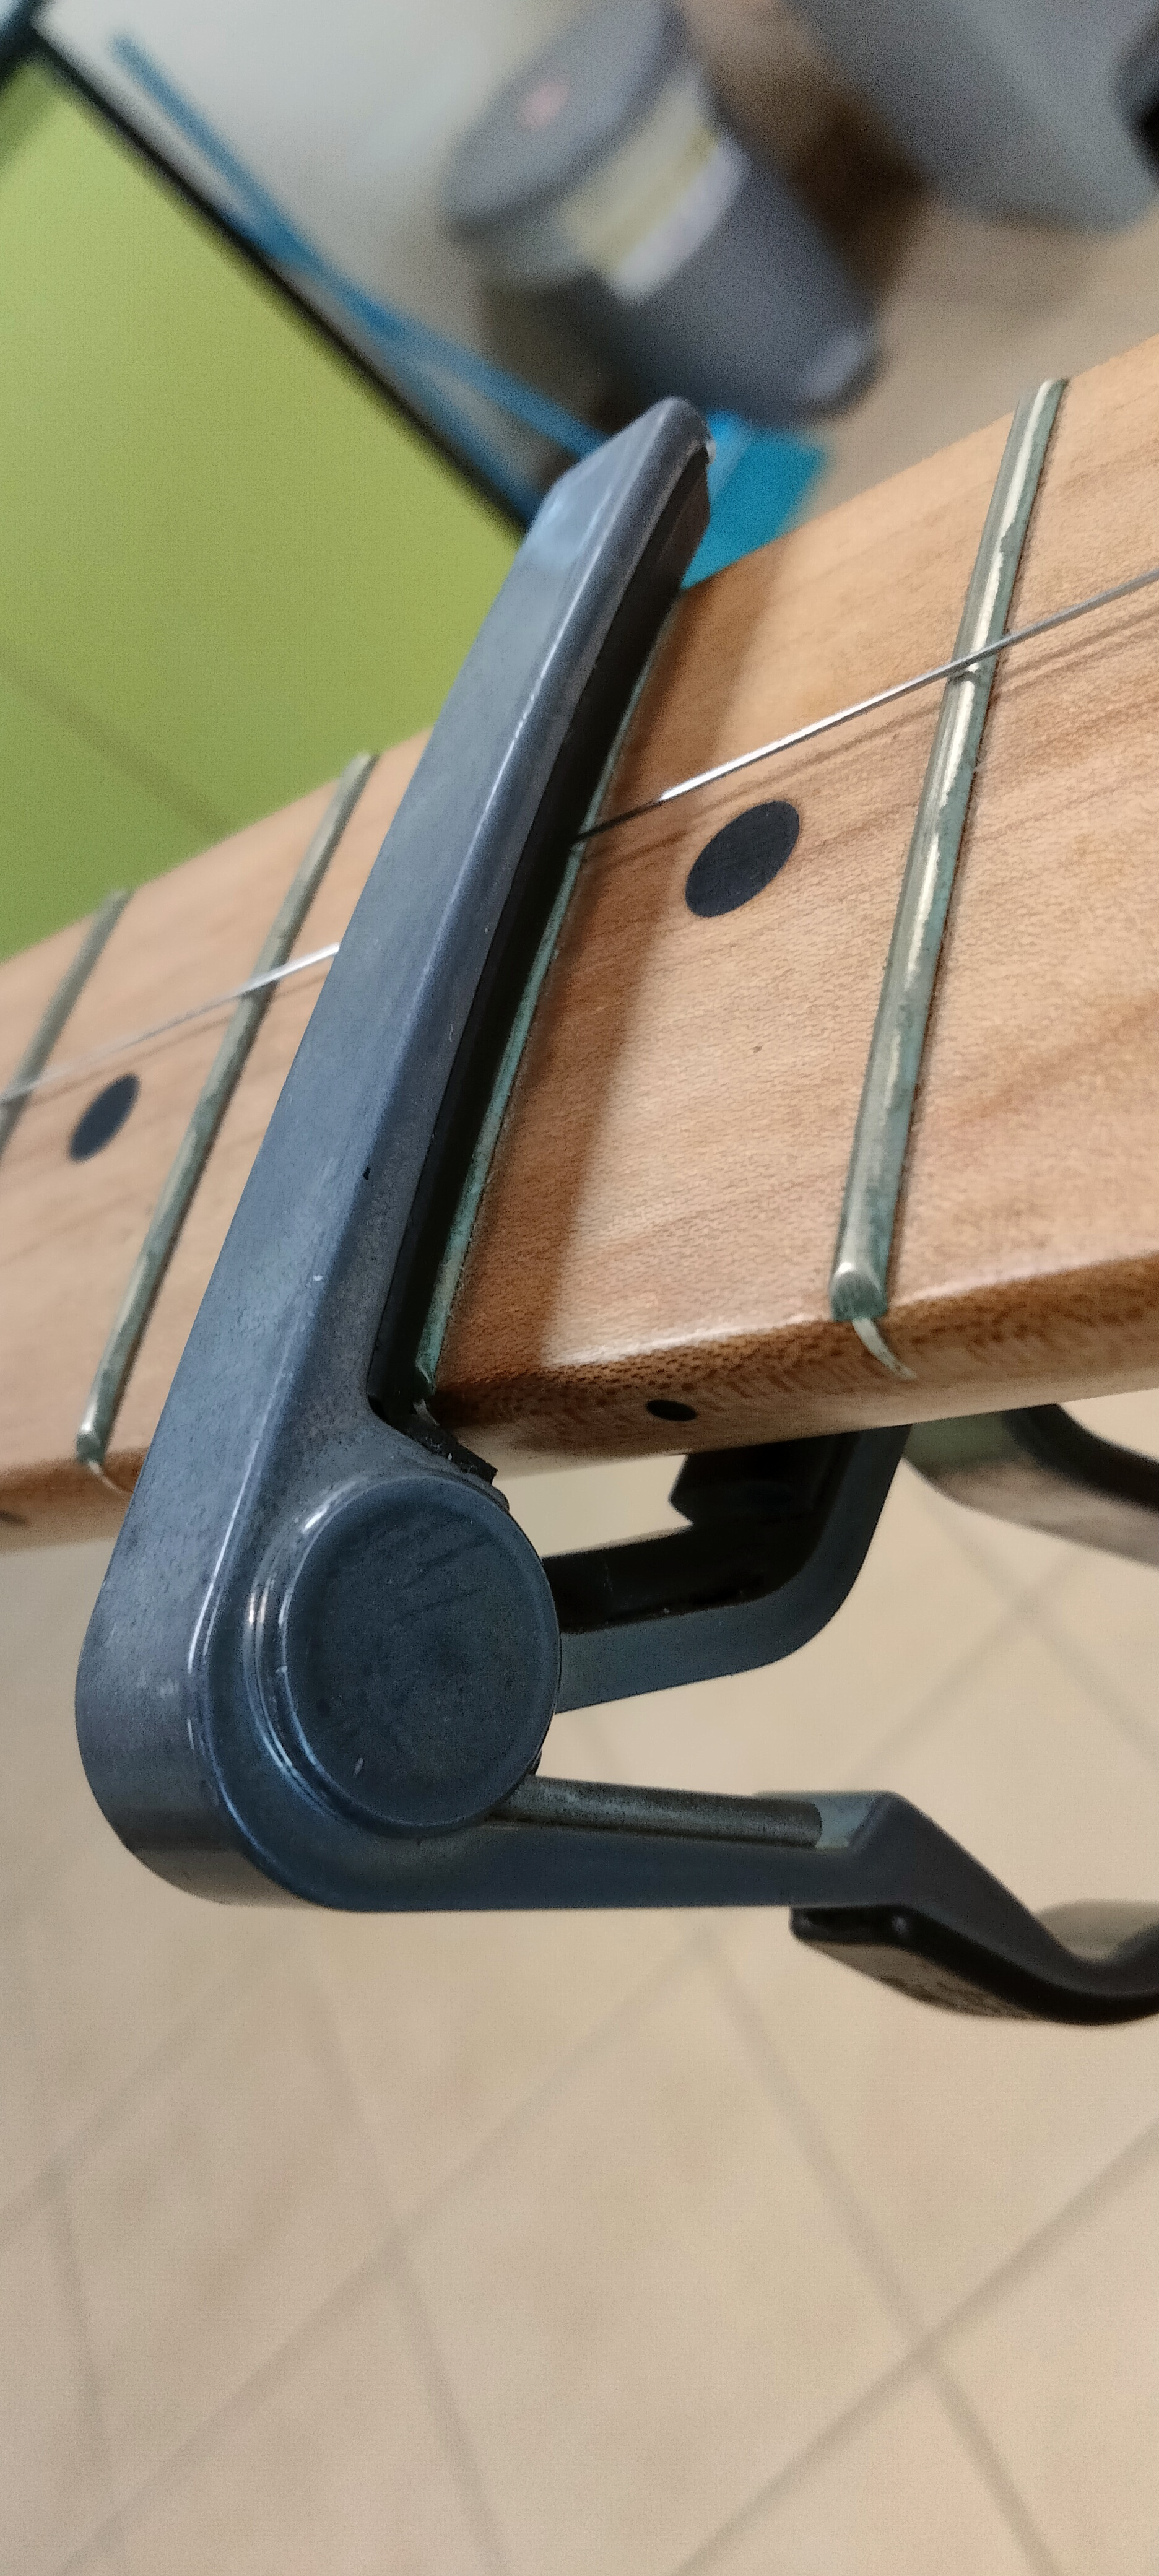
\includegraphics[angle=270, width = \textwidth]{ee/capo_on_fret.jpg}
    \caption{Close up of capo placement. This ensures consistent pressure and contact with the string and fret} \label{fig6}
\end{figure}
\begin{figure}[!htb]
    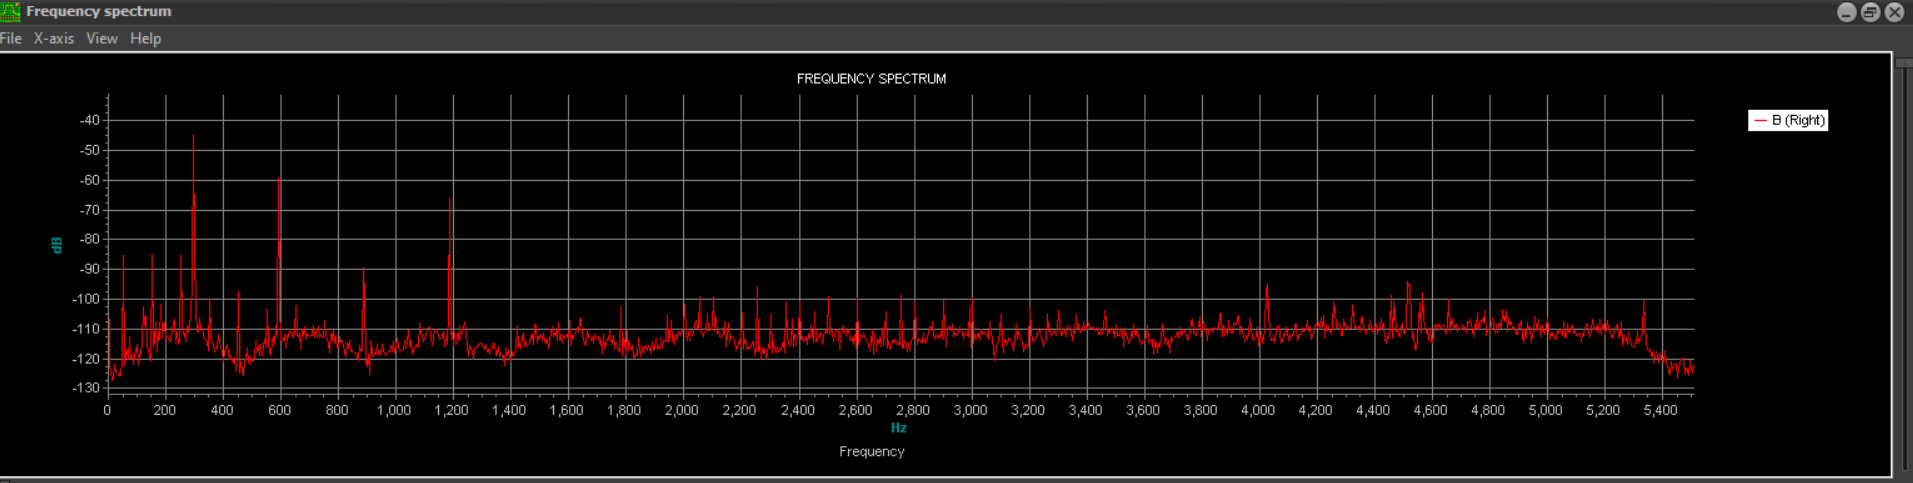
\includegraphics[width = \textwidth]{./ee/freq.png}
    \caption{Frequency spectrum of a note in Visual Analyzer. This can be zoomed in further to accurately read peak frequency value.} \label{fig7}
\end{figure}
\FloatBarrier